\documentclass[12pt, a4paper]{article}

\usepackage[utf8]{inputenc}
\usepackage[T1]{fontenc}
\usepackage[brazil]{babel}
\usepackage{geometry}
\geometry{a4paper, margin=3cm}
\usepackage{graphicx}
\usepackage{amsmath}
\usepackage{booktabs}
\usepackage{hyperref}
\usepackage{cite}
\usepackage{xcolor}

\hypersetup{
    colorlinks=true,
    linkcolor=blue,
    filecolor=magenta,
    urlcolor=cyan,
    citecolor=blue,
}

\title{
    \vspace{-1.5cm}
    \textbf{Desenvolvimento de Sistema Automatizado para Limpeza e Arrefecimento de Painéis Fotovoltaicos (ASCM)}
}

\author{    
    César Kerber \\
    Lucas Ekroth \\
    Paulo Rangel \\
    \vspace{0.2cm}
    \small Curso de Engenharia de Controle e Automação \\
    \small Instituto Federal de Educação, Ciência e Tecnologia de São Paulo (IFSP) \\
    \small Orientador: Prof. Valdeci Donizete Gonçalves
}

\date{\today}

\begin{document}

\maketitle

\begin{abstract}
\noindent A eficiência de sistemas solares fotovoltaicos é severamente afetada por fatores ambientais externos, sendo o acúmulo de sujeira (\textit{soiling}) e o superaquecimento das células os dois principais fatores de perda de geração. Este trabalho apresenta o desenvolvimento de um protótipo de Sistema Automatizado de Limpeza e Arrefecimento de Painéis Fotovoltaicos (\textit{Automated Self-Cleaning and Cooling Mechanism} - ASCM). O sistema realiza a limpeza mecânica por meio de aspersão de água combinada com um rodo motorizado, e o resfriamento evaporativo por meio do acionamento de uma mini-bomba hidráulica. A lógica de controle é baseada em microcontrolador Arduino Uno rodando o protocolo Telemetrix, integrado a um backend Python (FastAPI) e a um dashboard em Streamlit para monitoramento em tempo real. O acionamento da limpeza é guiado de forma inteligente pela comparação diferencial de potência entre um painel principal e um painel de referência mantido limpo. Este artigo descreve a arquitetura eletromecânica, o desenvolvimento de software e estabelece a metodologia para os ensaios práticos de diminuição de eficiência e validação térmica a serem conduzidos com o protótipo completo.
\end{abstract}

\textbf{Palavras-chave:} Energia Solar Fotovoltaica. Soiling. Arrefecimento Térmico. Automação. Arduino.

\newpage

\section{Introdução}

A transição energética global em direção a fontes renováveis tem posicionado a energia solar fotovoltaica como um dos pilares fundamentais da matriz elétrica de diversos países. Segundo relatórios da organização de estudos energéticos \textit{Ember} \cite{ember_brazil_2024, ember_eu_2026}, o Brasil alcançou a marca histórica em que a geração eólica e solar fotovoltaica combinadas ultrapassam um terço da eletricidade produzida no país \cite{ember_brazil_2024}, conforme ilustrado na Figura \ref{fig:grafico_ember}. Paralelamente, na União Europeia, as fontes renováveis atingiram cerca de 30\% da matriz elétrica \cite{ember_eu_2026}. Com o crescimento exponencial da capacidade instalada, torna-se crítico assegurar que esses ativos operem com o máximo aproveitamento energético possível.

\begin{figure}[htbp]
    \centering
    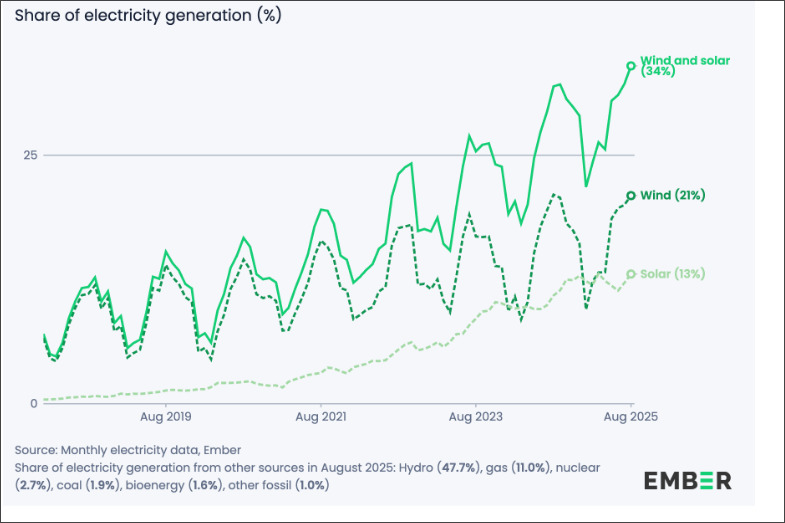
\includegraphics[width=0.65\textwidth]{images/grafico_ember.png}
    \caption{Geração elétrica renovável no Brasil, evidenciando o crescimento de eólica e solar.}
    \label{fig:grafico_ember}
    \centerline{\small Fonte: Adaptado de Ember (2024).}
\end{figure}

Apesar dos avanços tecnológicos nos materiais semicondutores, a eficiência operacional de um módulo fotovoltaico é drasticamente degradada por variáveis externas em campo. O primeiro fator crítico é o acúmulo de poeira, pólen, dejetos e poluentes suspensos no ar na superfície de vidro do painel, fenômeno conhecido na literatura como \textit{soiling} \cite{qi2025}. A poeira depositada obstrui a radiação solar direta que penetra nas junções p-n, diminuindo a corrente gerada. Estudos apontam que o acúmulo contínuo de poeira pode reduzir a eficiência do painel em até 7,84\% por semana em locais de alta taxa de deposição, podendo ultrapassar 50\% de perda total em períodos de seca prolongada sem intervenção humana ou precipitações pluviométricas de volume adequado \cite{qi2025}. O impacto negativo do acúmulo de sujidade na potência máxima de saída das células fotovoltaicas está quantificado graficamente na Figura \ref{fig:grafico_soiling}.

\begin{figure}[htbp]
    \centering
    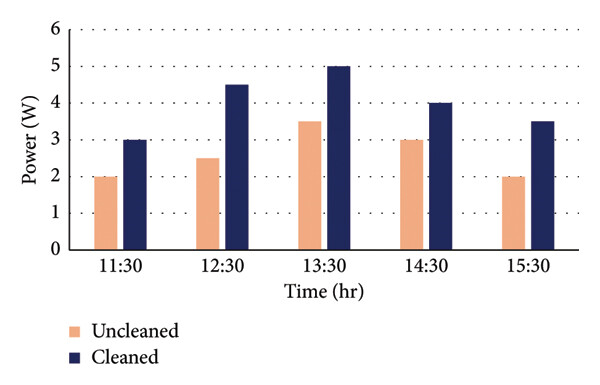
\includegraphics[width=0.55\textwidth]{images/grafico_soiling.jpg}
    \caption{Gráfico representativo das perdas na potência de saída em função da deposição de poeira ao longo de períodos secos.}
    \label{fig:grafico_soiling}
    \centerline{\small Fonte: Adaptado de Qi et al. (2025).}
\end{figure}

O segundo fator crítico relaciona-se ao coeficiente de temperatura do silício. O aquecimento natural do painel solar devido à radiação térmica eleva a temperatura de operação muito acima dos 25$^\circ$C padronizados em laboratório. Para cada grau Celsius acrescido à superfície, a potência máxima de saída do painel decresce linearmente entre 0,5\% e 0,6\% \cite{geetha2024}. A deposição de poeira agrava este quadro por atuar como isolante térmico local, mantendo o calor aprisionado sob a camada de sujeira e acelerando a degradação e o envelhecimento do módulo.

Neste cenário, soluções que combinem limpeza automática e arrefecimento ativo demonstram alto potencial técnico e econômico. O presente artigo detalha o desenvolvimento do sistema ASCM, estruturado com foco em baixo custo, sensoriamento em tempo real e facilidade de manutenção mecânica. Adicionalmente, apresenta-se o plano de ensaios práticos que serão executados após a montagem final do protótipo físico para quantificar a taxa exata de atenuação de eficiência do painel e avaliar o desempenho térmico de resfriamento.

\section{Referencial Teórico e Estado da Arte}

\subsection{Mecanismos de Limpeza Ativa e Passiva}

A literatura científica classifica os métodos de higienização de painéis fotovoltaicos em duas principais categorias:
\begin{itemize}
    \item \textbf{Métodos Passivos (Revestimentos):} Utilizam nanotecnologia aplicada à superfície do vidro para formar películas super-hidrofóbicas. Esses revestimentos diminuem o ângulo de contato da água e reduzem as forças de adesão de Van der Waals das partículas de poeira \cite{qi2025}. Embora promissores, apresentam custo elevado de aplicação e vida útil curta sob intempéries e abrasão mecânica.
    \item \textbf{Métodos Ativos (Mecânicos e Pneumáticos):} Compreendem sistemas que despendem energia para a remoção da poeira. Os robôs autônomos utilizam esteiras e escovas rotativas para transladar entre painéis. Entretanto, sua complexidade e custo são proibitivos para instalações de pequeno e médio porte. Os sistemas de aspersão com bicos aspersores combinados a rodos motorizados (\textit{wipers}) destacam-se pelo equilíbrio entre custo de instalação e alta eficácia. Estudos práticos realizados por Geetha et al. \cite{geetha2024} indicaram um aumento real de 14,81\% na potência de saída utilizando esta abordagem de aspersão com limpeza mecânica controlada por microcontrolador.
\end{itemize}

\subsection{O Fenômeno de Cristalização de Sujeira (\textit{Dust Scaling})}

Estudos de Qi et al. \cite{qi2025} apontam que a interação da poeira seca com a umidade do ar (como o orvalho matinal) é responsável pelo fenômeno de \textit{dust scaling} ou formação de crosta rígida (\textit{hard scale}). Quando a umidade relativa situa-se na faixa entre 40\% e 80\%, formam-se pontes de água microscópicas por capilaridade entre as partículas de poeira e o vidro. Após o nascer do sol e subsequente evaporação da água, sais minerais solúveis cristalizam-se, cimentando a sujeira na superfície. A remoção de tal camada torna-se inviável por meio de métodos puramente a seco (como sopro de ar ou escovação seca simples), exigindo o uso controlado de água como solvente mecânico aliado ao atrito de um rodo.

\subsection{Gestão Hídrica}

Um desafio frequente na higienização por aspersão é o consumo de água, elemento que pode impactar negativamente a sustentabilidade ecológica e econômica do projeto. Autores como Cavalcante et al. \cite{cavalcante2016} propõem a implementação de captação de água pluvial conjugada a filtros físicos de sedimentação e filtragem de partículas grossas e finas no reservatório do próprio sistema fotovoltaico. Tal abordagem reduz o consumo líquido de água potável da rede de distribuição a níveis próximos de zero, viabilizando o sistema para regiões semiáridas ou remotas.

\section{Metodologia e Arquitetura do ASCM}

O protótipo do sistema ASCM foi desenvolvido utilizando componentes comerciais de prateleira (COTS - \textit{Commercial Off-The-Shelf}) visando manter a replicabilidade e o baixo custo de fabricação. A arquitetura divide-se nas seções de Hardware, Software de Supervisão e Estratégia de Controle.

\subsection{Especificação e Arquitetura de Hardware}

O hardware eletrônico está centrado no microcontrolador Arduino Uno R3. A pinagem completa e o barramento do protótipo estão estruturados conforme detalhado no Guia de Hardware \cite{electronics_guide}. As conexões principais consistem em:
\begin{itemize}
    \item \textbf{Aquisição de Potência Elétrica (Sensores INA219):} Dois módulos INA219 integrados via barramento de comunicação $I^2C$ realizam a medição bidirecional de corrente e tensão. O sensor principal (endereço original $0x40$) monitora o painel limpo pelo sistema. O segundo sensor (endereço $0x41$, configurado via ponte de solda no pino de endereço A0) monitora o painel de referência, que permanecerá exposto ao acúmulo de sujeira natural. Ambas as saídas dos painéis são aplicadas sobre resistores de carga de 33 $\Omega$ e potência mínima de 1.5W para simular o consumo constante de carga.
    \item \textbf{Sensoriamento de Condições Ambientais:} Um sensor analógico de luz (resistor dependente de luz - LDR) associado a um divisor de tensão de 10 k$\Omega$ é lido pela porta analógica A0 para estimar a irradiância luminosa relativa. A medição térmica da superfície do painel é realizada por meio de um termopar LM35 montado na face traseira do painel, lido pela porta analógica A1.
    \item \textbf{Atuadores Eletromecânicos:} O rodo mecânico é movido linearmente por um motor de corrente contínua (DC) acoplado a uma redução mecânica. O acionamento da velocidade do motor é feito via sinal PWM pelo pino 11, e o sentido de movimentação é comandado pelos pinos digitais 9 e 10 de um driver Ponte H L298N. Chaves fim de curso do tipo \textit{micro-switch} estão instaladas no início (pino digital 2, \textit{Home}) e fim (pino digital 3, \textit{End}) do trilho de deslizamento.
    \item \textbf{Subsistema Hidráulico:} Consiste em uma mini-bomba d'água submersível de 5V controlada via driver L298N (pino PWM 6 para fluxo e pinos digitais 7 e 8 para sentido/ativação) ligada a bicos aspersores instalados no topo do painel principal para nebulizar o fluido na superfície do vidro.
\end{itemize}

A alimentação de energia da ponte H é provida de forma externa por uma fonte de alimentação CC de 5V dedicada para motores e bomba, compartilhando a mesma referência de terra (GND) com o microcontrolador Arduino. O diagrama de conexões elétricas e esquemático do protótipo eletrônico de montagem está ilustrado na Figura \ref{fig:diagrama_eletronica}.

\begin{figure}[htbp]
    \centering
    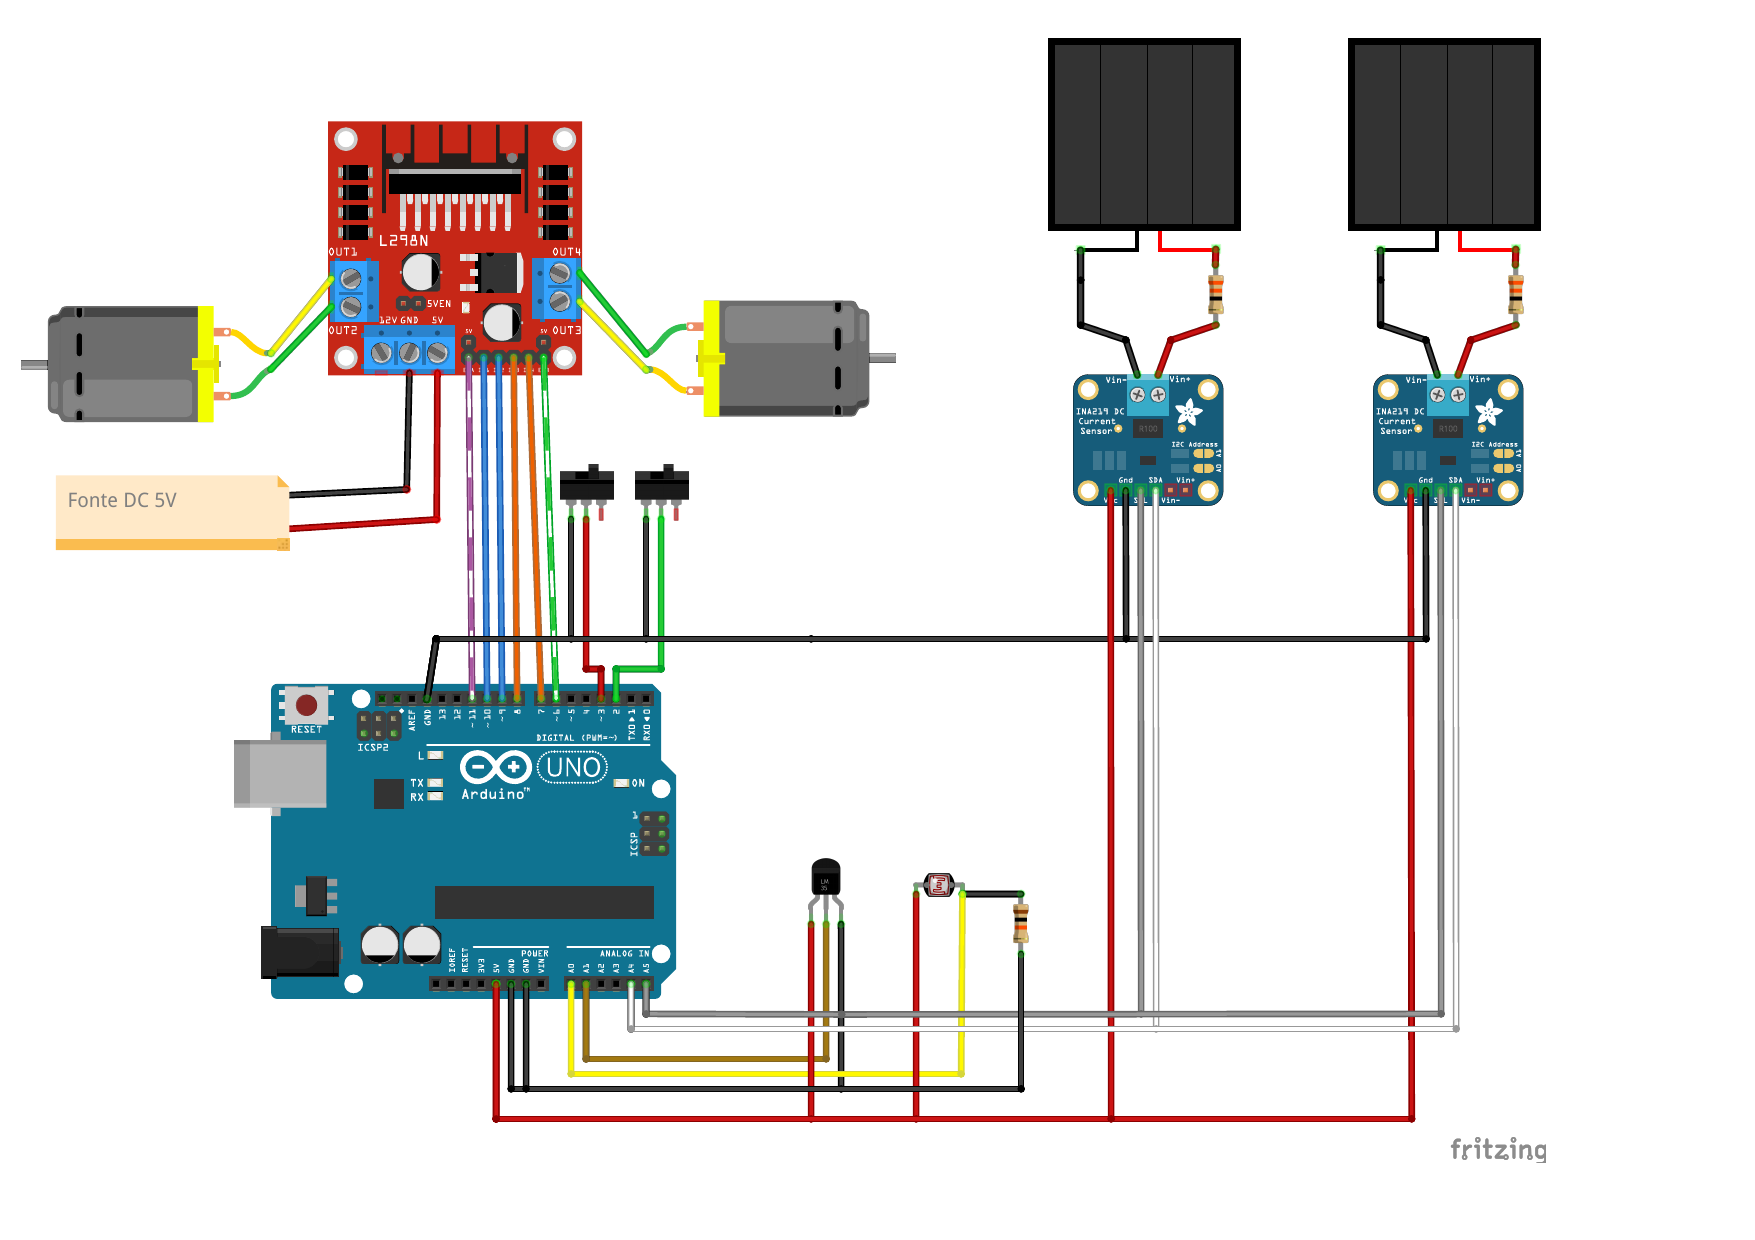
\includegraphics[width=0.7\textwidth]{images/diagrama_eletronica.png}
    \caption{Diagrama de conexões elétricas e esquemático de montagem física dos componentes eletrônicos do ASCM.}
    \label{fig:diagrama_eletronica}
    \centerline{\small Fonte: Elaborado pelos autores.}
\end{figure}

\subsection{Design Mecânico e Modelagem 3D}

O design estrutural e o mecanismo de movimentação linear do ASCM foram totalmente modelados utilizando o software de CAD tridimensional Autodesk Inventor, visando a prototipagem rápida através da fabricação por manufatura aditiva (impressão 3D por deposição de material fundido - FDM). O design mecânico compreende a modelagem dos seguintes componentes principais:
\begin{itemize}
    \item \textbf{Chassi Estrutural (Frame):} Estrutura que suporta os dois painéis solares em um ângulo de inclinação fixo otimizado para a irradiância solar da região geográfica e para o escoamento de água por gravidade.
    \item \textbf{Mecanismo de Transmissão por Pinhão e Cremalheira (Gear and Rack):} Para evitar deslizamentos mecânicos comuns em transmissões por polia e correia sob condições de umidade e exposição direta a respingos de água, o sistema adota um mecanismo de pinhão e cremalheira. A cremalheira (\textit{Gear-Rack}) é fixada ao longo das guias lineares do frame, e o pinhão (\textit{Gear} acoplado ao eixo do motor DC) engrena diretamente na cremalheira para guiar a translação suave do rodo.
    \item \textbf{Suporte do Rodo (Wiper Support):} Peça personalizada que aloja o motor de tração com redução e fixa a haste do rodo de silicone contra a superfície do vidro do painel principal, garantindo uma pressão de contato uniforme para a varredura da poeira.
    \item \textbf{Suporte de Aspersão (Sprinkler Support):} Fixadores posicionados no topo do painel que sustentam a tubulação hidráulica e os bicos aspersores orientados em ângulo que maximiza a área de cobertura da lâmina d'água na superfície.
    \item \textbf{Suportes dos Painéis (Panel Support):} Peças de interface que prendem os módulos fotovoltaicos de forma rígida ao frame estrutural principal.
\end{itemize}
A modelagem em CAD de todas as peças foi exportada em formato STL para fabricação por manufatura aditiva. Para a confecção do protótipo físico de teste, utilizou-se filamento de PLA (Ácido Polilático) pela facilidade de prototipagem rápida e baixo custo, embora materiais como PETG ou ABS possam ser aplicados em versões finais expostas a intempéries contínuas caso o equipamento de impressão ofereça suporte a tais polímeros. O modelo tridimensional do chassi completo, o segmento da cremalheira linear e o suporte do rodo motorizado estão ilustrados nas Figuras \ref{fig:frame_cad}, \ref{fig:cremalheira_cad} e \ref{fig:wiper_cad}.

\begin{figure}[htbp]
    \centering
    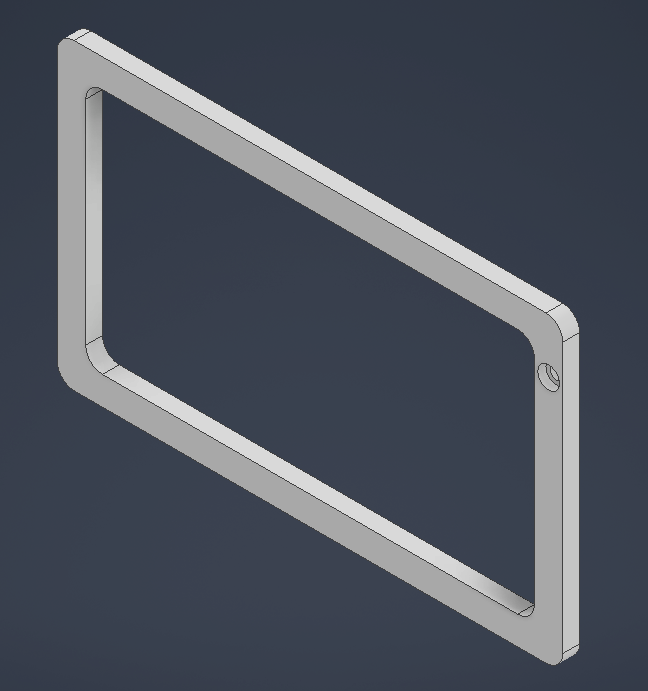
\includegraphics[width=0.55\textwidth]{images/frame_cad.png}
    \caption{Modelo tridimensional (CAD) do chassi estrutural (Frame) completo do ASCM no Autodesk Inventor.}
    \label{fig:frame_cad}
    \centerline{\small Fonte: Elaborado pelos autores.}
\end{figure}

\begin{figure}[htbp]
    \centering
    
\includegraphics[width=0.55\textwidth]{images/cremalheira_cad.png}
    \caption{Detalhe da cremalheira linear (Gear Rack) projetada em CAD.}
    \label{fig:cremalheira_cad}
    \centerline{\small Fonte: Elaborado pelos autores.}
\end{figure}

\begin{figure}[htbp]
    \centering
    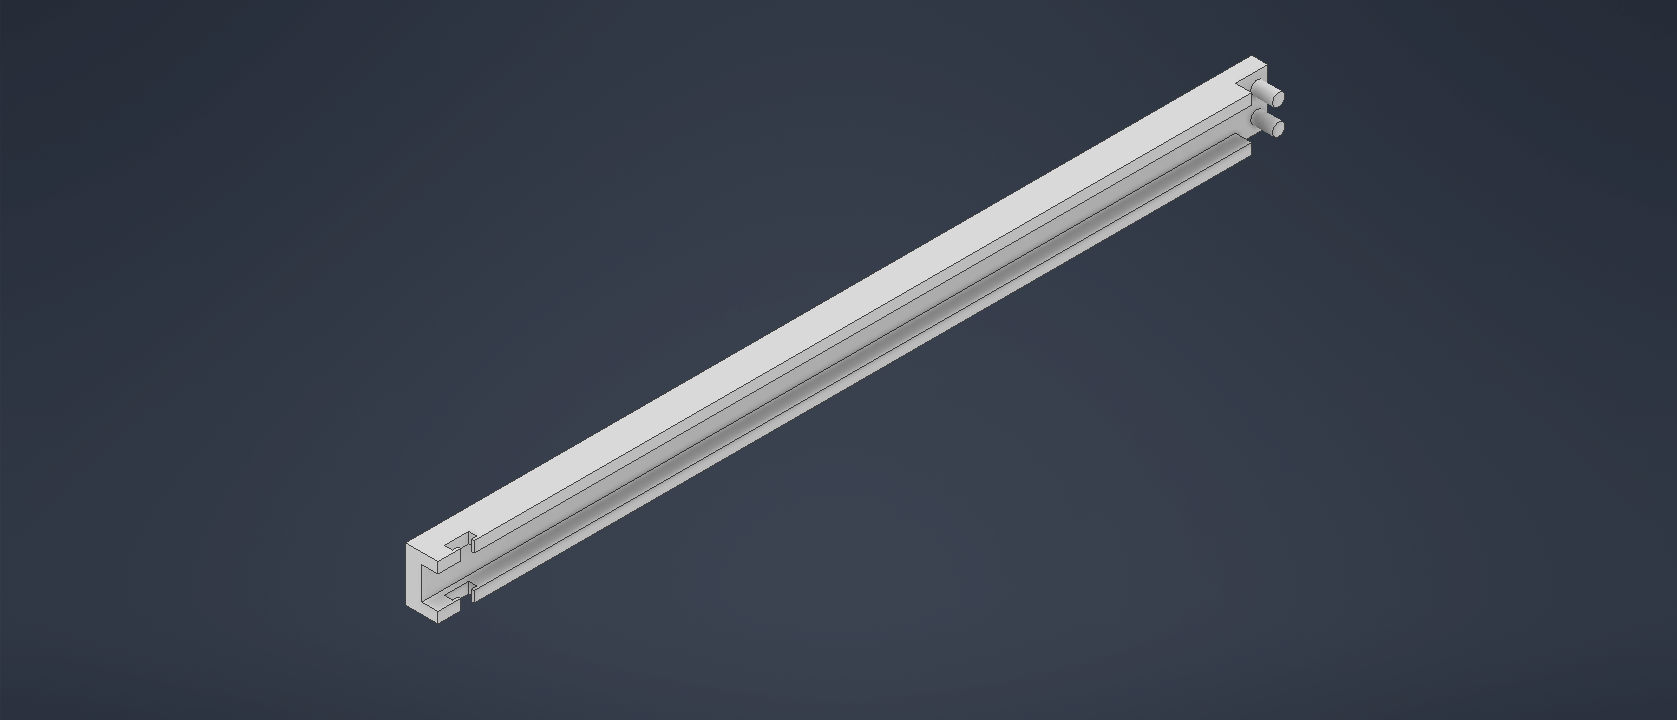
\includegraphics[width=0.55\textwidth]{images/wiper_cad.png}
    \caption{Modelo tridimensional do suporte do rodo motorizado (Wiper Support) e acoplamento do motor com o pinhão.}
    \label{fig:wiper_cad}
    \centerline{\small Fonte: Elaborado pelos autores.}
\end{figure}

\subsection{Arquitetura do Software e Comunicação}

Ao contrário de abordagens convencionais com firmware C/C++ estático compilado no Arduino, o ASCM adota a arquitetura **Telemetrix** \cite{telemetrix_ref}. O Arduino Uno executa o sketch padrão \textit{Telemetrix4Arduino}, operando puramente como um dispositivo escravo de entrada e saída (servidor de I/O) que se comunica via porta serial com um computador hospedeiro. 

Toda a lógica de controle complexa, o tratamento matemático e os logs são implementados na linguagem Python no computador servidor:
\begin{enumerate}
    \item \textbf{Backend (FastAPI):} Desenvolve o controle centralizado de eventos e automatiza o laço periódico. Ele atualiza leituras analógicas e digitais usando callbacks rápidos implementados no Telemetrix, e interroga os sensores $I^2C$ de potência INA219. O laço síncrono também interage com uma API de meteorologia online para coletar a temperatura ambiente local e checar a incidência de chuvas no momento. Os logs de telemetria e eventos são exportados periodicamente para arquivos CSV estruturados.
    \item \textbf{Frontend (Streamlit):} Provê uma interface web simplificada para o monitoramento instantâneo do sistema. O dashboard apresenta de forma intuitiva as grandezas elétricas de geração (tensão, corrente, potência), a temperatura da superfície e a diferença percentual de rendimento devido ao \textit{soiling}, além de permitir comandos manuais de emergência (parada total, ativação forçada de bomba ou motor).
\end{enumerate}

\subsection{Estratégia do Laço de Controle Automatizado}

A estratégia de automação funciona em ciclo contínuo em segundo plano e adota dois gatilhos paralelos e complementares:
\begin{enumerate}
    \item \textbf{Algoritmo de Resfriamento Térmico:} A temperatura da superfície do painel fotovoltaico ($T_{painel}$) é medida pelo termopar LM35 e comparada com a temperatura ambiente real ($T_{amb}$) retornada pelo serviço de meteorologia. O resfriamento é disparado se:
    \begin{equation}
        T_{painel} > T_{amb} + \Delta T_{lim}
    \end{equation}
    onde $\Delta T_{lim}$ é o diferencial limite definido no sistema (padrão de 5$^\circ$C). A bomba de água é acionada em modo de fluxo alto por um período programado até que a temperatura do painel se estabilize abaixo do limiar.
    \item \textbf{Algoritmo de Higienização de Sujeira:} A potência gerada pelo painel principal ($P_{main}$) e pelo painel de referência dirty ($P_{ref}$) são calculadas pelos respectivos sensores de potência INA219. A perda percentual por \textit{soiling} ($\Delta \eta$) é dada por:
    \begin{equation}
        \Delta \eta = \left( \frac{P_{ref} - P_{main}}{P_{ref}} \right) \times 100\%
    \end{equation}
    Se $\Delta \eta > \eta_{lim}$ (onde $\eta_{lim}$ é o limiar de sujeira tolerado, tipicamente 10\%) e a API de clima indicar que não há precipitação de chuva em andamento, o backend FastAPI invoca a tarefa assíncrona de ciclo de limpeza completo:
    \begin{itemize}
        \item Ativação da bomba d'água em fluxo baixo para molhar a poeira e amolecer o \textit{hard scale} por 2 segundos.
        \item Deslocamento do rodo mecânico na direção progressiva (\textit{forward}) com velocidade controlada via PWM até atingir a chave fim de curso final (\textit{limit\_end}).
        \item Breve pausa de 1 segundo e subsequente reversão do motor na direção contrária (\textit{backward}) até pressionar a chave fim de curso inicial (\textit{limit\_home}).
        \item Desligamento do motor e da bomba hidráulica, retornando o sistema ao monitoramento em malha fechada.
    \end{itemize}
\end{enumerate}

A lógica de funcionamento integrada de controle periódico, monitoramento de limites e acionamentos automáticos baseados nas decisões térmicas e de sujeira é apresentada no fluxograma de controle da Figura \ref{fig:fluxograma_controle}.

\begin{figure}[htbp]
    \centering
    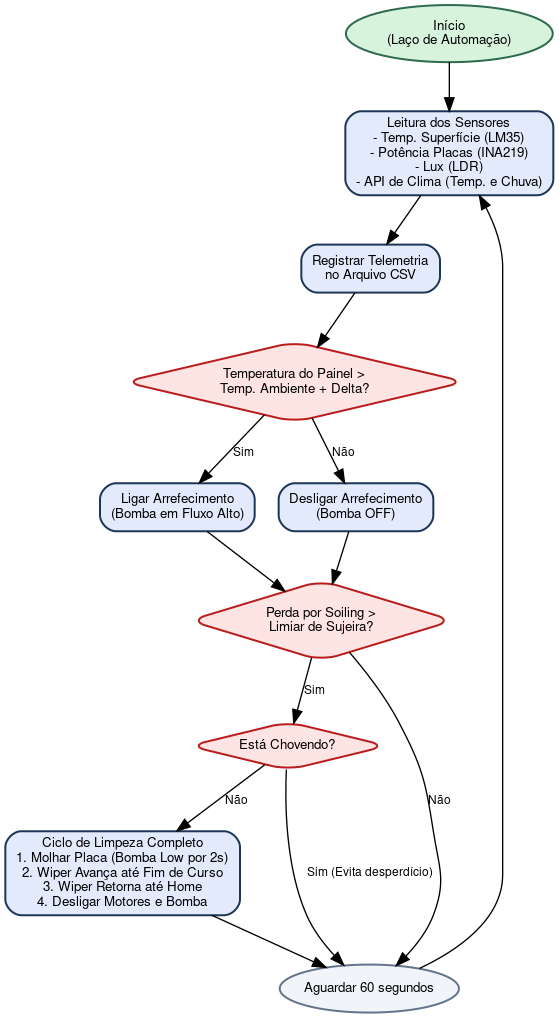
\includegraphics[width=0.55\textwidth]{images/fluxograma.png}
    \caption{Fluxograma do laço de controle de automação e de tomada de decisão do sistema ASCM.}
    \label{fig:fluxograma_controle}
    \centerline{\small Fonte: Elaborado pelos autores.}
\end{figure}

\section{Resultados Preliminares e Metodologia de Ensaios}

Esta seção descreve a validação inicial do software de controle e detalha a metodologia projetada para os futuros ensaios empíricos com o protótipo físico completo montado.

\subsection{Validação do Loop de Automação de Software}

Durante as simulações do software de controle, as rotinas de callback do Telemetrix integradas à biblioteca FastAPI demonstraram latência inferior a 15 ms para detecção das chaves fim de curso, garantindo uma parada de emergência segura para os motores de movimentação linear do rodo. As leituras em barramento compartilhado dos sensores INA219 a frequências de amostragem de 1 Hz mostraram-se estáveis, com flutuações de corrente e tensão inferiores a 1,2\%, adequadas para o cálculo preciso do rendimento diferencial.

\subsection{Metodologia para Ensaio Físico e Acúmulo de Poeira (\textit{Soiling})}

Com a montagem do protótipo físico completo em andamento, será conduzido um ensaio experimental com o objetivo de levantar a curva de diminuição da eficiência energética devido ao acúmulo de sujeira. O procedimento do ensaio seguirá as seguintes etapas:
\begin{enumerate}
    \item Ambos os painéis (principal e referência) serão instalados externamente em suporte ajustável, expostos sob as mesmas condições de inclinação, orientação geográfica e sombreamento.
    \item No dia inicial ($t=0$), ambos os painéis serão limpos manualmente com água deionizada para garantir calibração inicial idêntica ($P_{main} \approx P_{ref}$).
    \item O painel de referência será mantido sob exposição ao acúmulo natural de poeira local por um período contínuo de 30 dias, sem passar por nenhum ciclo de limpeza automática.
    \item O painel principal passará pela automação do ASCM, disparando ciclos de limpeza sempre que a diferença de potência ultrapassar o limiar programado ($\eta_{lim} = 10\%$).
    \item Os parâmetros de geração (tensão, corrente, potência de pico e energia diária acumulada) serão registrados minuto a minuto para ambos os painéis. A irradiância local relativa será monitorada via LDR.
\end{enumerate}

\subsection{Placeholder para Resultados Experimentais Futuros}

A Tabela \ref{tab:ensaio_soiling} apresenta o modelo estrutural de dados que será preenchido para documentar a atenuação de eficiência e avaliar os ganhos trazidos pelo acionamento periódico do sistema ASCM.

\begin{table}[htbp]
    \centering
    \caption{Estrutura de dados para o ensaio de degradação por \textit{soiling} (a ser preenchida após ensaio).}
    \label{tab:ensaio_soiling}
    \begin{tabular}{cccccc}
    \toprule
    \textbf{Dia} & \textbf{Luminosidade (LDR)} & \textbf{Potência Principal ($P_{main}$)} & \textbf{Potência Ref. ($P_{ref}$)} & \textbf{Perda Diferencial ($\Delta \eta$)} & \textbf{Status da Limpeza} \\
    \midrule
    0 & --- & [A ser inserido] & [A ser inserido] & 0.0\% & Calibrado \\
    5 & --- & [A ser inserido] & [A ser inserido] & [A ser inserido] & --- \\
    10 & --- & [A ser inserido] & [A ser inserido] & [A ser inserido] & --- \\
    15 & --- & [A ser inserido] & [A ser inserido] & [A ser inserido] & --- \\
    20 & --- & [A ser inserido] & [A ser inserido] & [A ser inserido] & --- \\
    25 & --- & [A ser inserido] & [A ser inserido] & [A ser inserido] & --- \\
    30 & --- & [A ser inserido] & [A ser inserido] & [A ser inserido] & Finalizado \\
    \bottomrule
    \end{tabular}
\end{table}

\subsection{Ensaio de Arrefecimento e Ganho de Potência por Resfriamento}

Além do ensaio de sujidade, o termopar LM35 em conjunto com a bomba aspersora possibilitará a realização do ensaio térmico. Sob irradiância solar máxima no período do meio-dia (onde o painel atinge temperaturas elevadas superiores a 50$^\circ$C), o resfriamento evaporativo será acionado. Será mapeada a curva de queda de temperatura vs o ganho de potência instantânea resultante. Os resultados esperados, embasados na literatura, preveem uma redução térmica estável de 5$^\circ$C a 10$^\circ$C na temperatura de operação das células, correspondendo a uma recuperação linear de potência entre 2.5\% e 6.0\% no instante de resfriamento.

\section{Conclusão e Próximos Passos}

O protótipo do ASCM projetado demonstrou-se viável sob o aspecto de desenvolvimento de software e integração de hardware de baixo custo, orçando um custo total de montagem inferior ao de soluções industriais. O uso do protocolo Telemetrix permitiu a criação de um laço de automação flexível e centralizado no computador hospedeiro via FastAPI e Streamlit.

Os próximos passos deste trabalho consistem no término do acoplamento mecânico estrutural do rodo impresso em 3D no painel solar físico e no início imediato dos ensaios de degradação por sujidade de 30 dias e testes térmicos. Espera-se com esses testes validar a eficácia prática da aspersão com raspagem mecânica na remoção de poeira consolidada (\textit{hard scale}) e no ganho líquido anual de geração elétrica do sistema.

\begin{thebibliography}{99}

\bibitem{ember_eu_2026}
EMBER.
\textit{European Electricity Review 2026}.
Disponível em: \url{https://ember-energy.org/latest-insights/european-electricity-review-2026/}. Acesso em: 24 mar. 2026.

\bibitem{ember_brazil_2024}
EMBER.
\textit{Wind and solar generate over a third of Brazil's electricity for the first month on record}.
Disponível em: \url{https://ember-energy.org/latest-insights/wind-and-solar-generate-over-a-third-of-brazils-electricity-for-the-first-month-on-record/}. Acesso em: 24 mar. 2026.

\bibitem{geetha2024}
GEETHA, A.; USHA, S.; SANTHAKUMAR, J.; PALANISAMY, R.; SARAWAGI, R.; SINGH, A. 
Solar Panel Self-Cleaning Mechanisms and Its Effect on the Economic and Environmental Sustainability. 
\textit{Journal of Electrical and Computer Engineering}, Hindawi, vol. 2024, Article ID 7726716, 2024.

\bibitem{qi2025}
QI, Jiacheng; DONG, Qichang; SONG, Ye; ZHAO, Xiaoqing; SHI, Long.
Combining dust scaling behaviors of PV panels and water cleaning methods. 
\textit{Renewable and Sustainable Energy Reviews}, Elsevier, vol. 212, 115394, 2025.

\bibitem{cavalcante2016}
CAVALCANTE, M. M.; MARCELINO, J. E. C.; DELGADO, D. B. M.; VIANA, E. C.
Protótipo de um sistema automatizado para higienização de painéis solares planos agrupado a um sistema de reaproveitamento de água. 
In: \textit{Anais do V SINGEP}, São Paulo – SP, Brasil, 2016.

\bibitem{electronics_guide}
ASCM Project Contributors.
\textit{Guia de Hardware Eletrônico - Instruções de Montagem}.
Disponível em: \url{hardware/Electronics/electronics.md}. Acesso em: 03 jun. 2026.

\bibitem{telemetrix_ref}
ASCM Project Contributors.
\textit{Firmware do Dashboard e Integração Telemetrix}.
Disponível em: \url{firmware/dashboard/backend/hardware.py}. Acesso em: 03 jun. 2026.

\end{thebibliography}

\end{document}
